\section{計測した反射強度の比較}

  計測した反射強度の比較を\figref{Fig:Comparison of reflection intensity by histogram}と\tabref{tab:Comparison of reflection intensity}に示す.
  これらの結果から,再帰反射テープよりも反射強度の高いものは存在せず,ルールベース制御器が正常に機能すれば,2DLiDARの反射強度を利用した人追従行動が可能であることを確認した.

  \vspace{0.5cm}

  \begin{figure}[h]
    \centering
    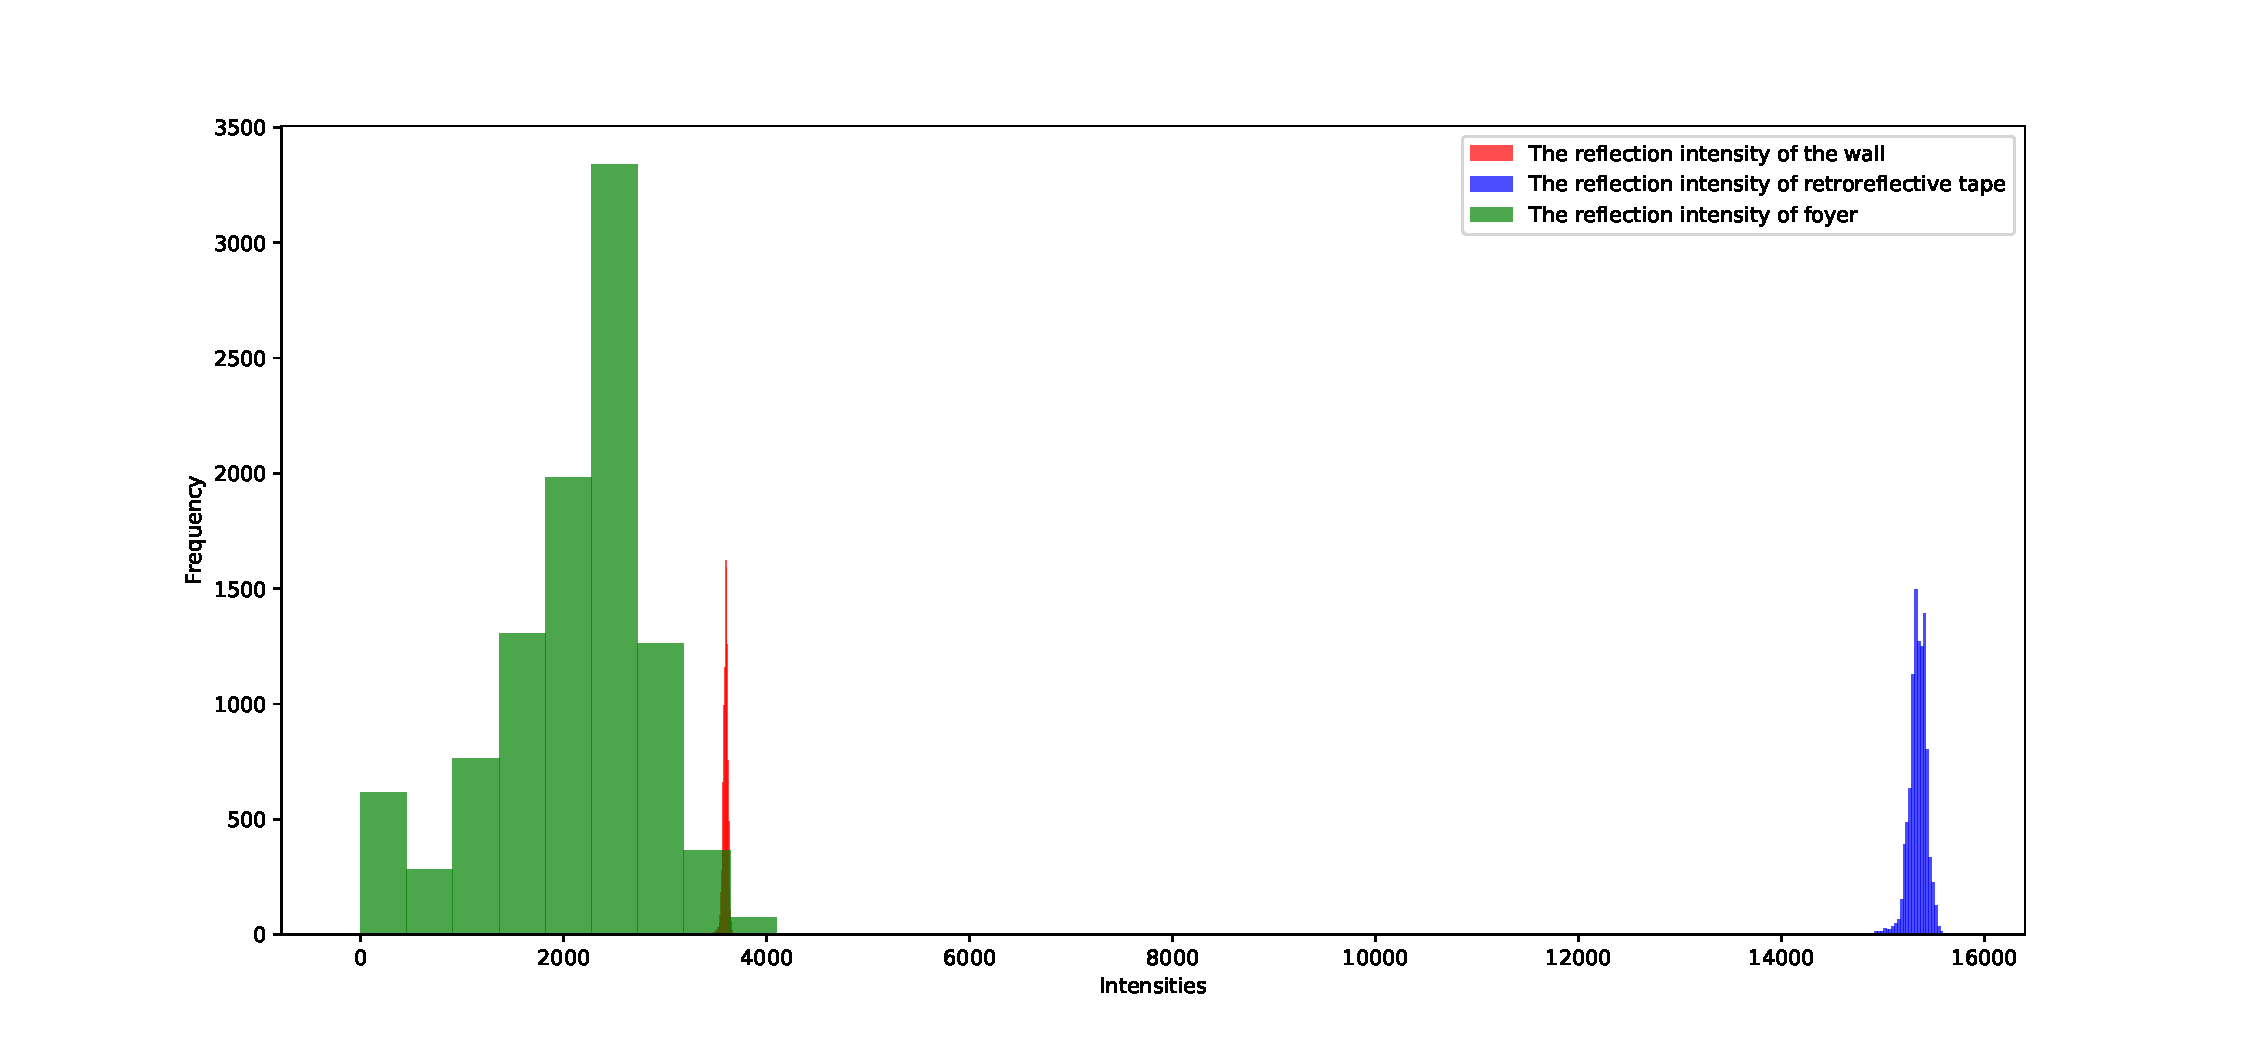
\includegraphics[width=14cm] {images/pdf/RobotGuidance_plot_reflection_intensities_of_all}
    \captionsetup{justification=raggedright} % キャプションを左寄せに
    \caption{Comparison of reflection intensity by histogram}
    \label{Fig:Comparison of reflection intensity by histogram}
  \end{figure}

  \vspace{0.5cm}

  \begin{table}[h]
    \caption{Comparison of reflection intensity}
    \label{tab:Comparison of reflection intensity}
    \centering
    \begin{tabular}{ccc}
    \hline
    Experiments                                      & Average & Variance \\
    \hline
    The reflection intensity of the wall             & 3600    & 546      \\
    The reflection intensity of retroreflective tape & 15300   & 7310     \\
    The reflection intensity of foyer                & 2102    & 676261  \\
    \hline
    \end{tabular}
  \end{table}

\newpage